\documentclass{jdrp}

\bibliography{songes-de-l-uhumele/references} 

\newcommand*{\crg}{{\aurebesh\Large \$}} % Symbol for Galactic Credits

\hypersetup{
	pdftitle={SWR - Songes de l’Uhumele},
	pdfsubject={Scénario, Songes de l’Uhumele},
	pdfauthor={Marthym},
	pdfkeywords={starwars,savage,worlds,jdr,scenario},
	pdfcopyright={This work is licensed under the Creative Commons Attribution-ShareAlike 4.0 International License.}
}

\begin{document}

	\begin{titlepage}

	\begin{center}
		\hspace*{\vfill}
		\noindent\Huge\jedifont{Star Wars Redemption}\\ 
		\noindent\fontsize{50}{70}\jedifont{\$}
		\noindent\fontsize{50}{70}\jedifont{\#}\\
		\noindent\fontsize{40}{60}\jedifont{Songes de l’uhumele}
		\hspace*{\vfill}
	\end{center}

	%\hspace*{\vfill}

	\noindent\makebox[\textwidth]{
		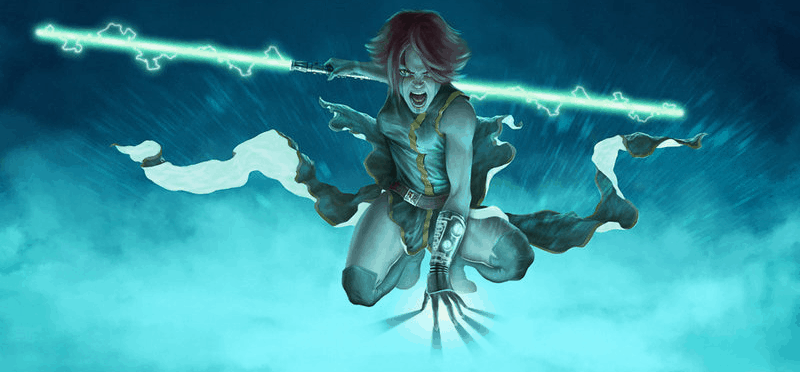
\includegraphics[width=\paperwidth]{_img/cover-bg.png}}
	\begin{tikzpicture}[overlay]
		\node[minimum width=200pt,minimum height=200pt] at (15,11){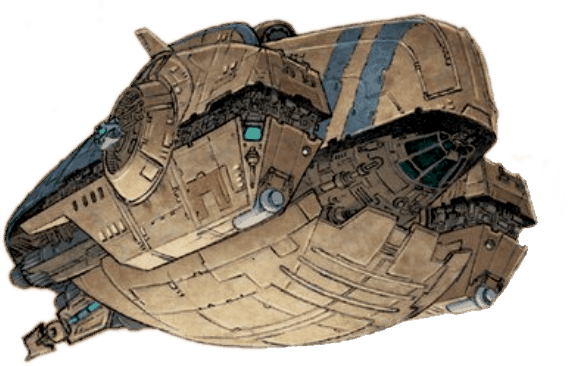
\includegraphics[width=240pt]{_img/songes-de-l-uhumele/uhumele.png}};
	\end{tikzpicture}}
	\end{titlepage}

	\onecolumn
	\section{Contexte du Scénario}
		\begin{wrapfigure}{R}{180pt}
			\centering
			
\includegraphics[width=180pt]{_img/songes-de-l-uhumele/bomo-greenbark.png}
			\caption{\label{fig:bomo-greenbark}Bomo Greenbark}
		\end{wrapfigure}

	Voici un court scénario sur le thème de \nameref{sec:uhumele}. Ce scénario bien qu’indépendant est fortement lié à la campagne "Dos au Muur" de \citetitle{jdrp-starwars}. C’est un scénario écrit pour pour faire patienter entre deux étapes de la campagne (2 et 3). 

	L’idée est que l’un des personages, sensible à la force et possédant \textit{Sens de Force} a une vision d’un évènement passé. En l’occurence, la tentative de sauvetage de Resa, la fille de \textbf{Bomo Greenbark} par l'équipage de l’Uhumele. Les joueurs jouent alors le rôle des membres de l’équipage (avec leur propre fiche de perso). Ce système à l’intéret d’introduire l’Uhumele dans la campagne Dos au Muur mais aussi de ne pas modifier les circonstances entre les 2 scénarios. Pas besoin de faire des raccords tiré par les cheveux.

	Biensûr, ce scénario peut aussi être joué hors du contexte de la campagne Dos au Muur, en remplaçant l’introduction "vision" par, par exemple, une introduction à base de contrat.

	A noter que ce scénario est plutôt fait pour des héros notre ou orienté gentils. 

	Ce scénario se passe normalement en -19 pendant les derniers affrontements entre l’armée des clones et les armées de droïde de la Confédération des Systèmes Indépendants.

	\twocolumn

	\section{introduction}
	L’équipage de \nameref{sec:uhumele} quitte Nouvelle Plympto au lendemain d’une grande bataille qui a obligé les habitants a évacuer pour se mettre à l’abri. \'A cette époque, l’équipage du Uhumele venait de mettre la main sur une cargaison inconnue et dangeureuse qui les pousse à éviter l’Empire au maximum. C’est pourquoi quand l’Empire est arrivé pour s’opposer aux droïdes, le vaisseau a quitté la planête en urgence. Mais dans la précipitation, la famille de \textbf{Bomo Greenbark} n’a pas eu le temps d’embarquer dans l’Uhumele et s'est trouvée évacuée par l’Empire. 

	Quand Bomo se renseigne pour savoir sur quel vaisseau a été évacué sa famille, il apprend que sa femme et sa fille ont embarqué sur le \textbf{Sevarog} un vaisseau à destination d’Orvax IV, plate-forme galactique majeure du trafic d’esclaves. Le scénario commence au moment où Bomo demande de l’aide à l’équipage de l’Uhumele pour récupérer sa fille.

	\section{orvax iv}
	Plate-forme galactique majeure du trafic d’esclaves, Orvax IV est situé dans la bordure extérieur et peuplé d’à peu près toutes les espèces que compte la galaxie. L’Empire comme la République ne s’y sont jamais intéressé et laisse cette planète faire ses affaire comme elle le souhaite.

	La planète se présente comme un vaste marché aux esclaves, trié en catégorie, races, age, genre, \ldots.

	Première étape, retrouver le \textbf{Sevarog} à bord duquel est arrivée la famille de Bomo. N’importe qui au spacioport donnera le numéro du quai où se trouve le vaisseau. Bien sur, les esclaves ont été débarqués et la famille de Bomo ne se trouve plus à bord. S’il l'interroge, le capitaine du Sevarog apprend que les esclaves déportés par l’Empire sont stocké dans un fosse au nord du spacioport en dessous de la boutique "U2".

	\section{Fosse u2}
	En tant qu’entrepot de stockage de l’Empire, la zone est sous bonne garde, des \nameref{sec:storm-trooper}s patrouilles régulièrement dans le coin et l’arrière de la boutique est gardé.

	Les héros ont le choix de passer par les égouts, de négocier ou de passer en force, a vous de doser la difficulté en fonction de leur niveau.

	Une fois arrivé dans le sous-sol de la boutique, les héros trouvent plusieurs fosses, grillagé sur le dessus, où s’entassent des centaines d’esclaves, majoritairement des femmes et des filles qui implorent pour qu'on les libère.

	Si les héros appellent Mesa ou Resa (la femme et la fille de Bomo), une des esclaves dans une fosse sur la droite sort la main de la grille et dit :

	\begin{quotebox}
    	Ici, ici, venez, je connais Mesa et Resa.

    	Faite moi sortir de là et je vous dirais où se trouve Mesa et Resa.
	\end{quotebox}
	Aux héros de voir comment ils gèrent ça. S’ils sont rentré en mode discrétion et qu’ils ressortent avec un ou plusieurs esclaves les jets de \textit{Discrétion} prennent un malus de \textbf{-2}. S’ils font sortir tous les esclaves, la \textit{Discrétion} n’est plus possible.

	Une fois que l’esclave se sent en sureté, elle leur explique que Resa a été vendu et que Mesa a été tuée en voulant s’interposer. Bomo est bouleversé et ses camarades doivent le retenir pour qu’il ne s’en prenne pas à l’esclave. Cette dernière se souvient du nom de l’acheteur, \textbf{Dezono Qua}, ce dernier a dit qu’il l’emmenait sur \textbf{Esseles}.

	\section{La forteresse d’Esseles}
	\textbf{Dezono Qua} est un humain excentrique et riche qui vit dans un forteresse miniature en haut d’une colline sur \textbf{Esseles}. Les autorités locales sont au courant que ses affaires ne sont pas toutes blanche mais sa fortune le tiens à l’abris des lois locales. Il vie seul dans sa forteresse protégée par une armée de droïdes.


	\section{Annexes}
	\subsection{l’Uhumele}\label{sec:uhumele}
	\onecolumn
	\subsection{Forteresse d’Esseles}\label{sec:forteresse-esseles}
	\begin{figure}[!h]
		\centering	
		\begin{tikzpicture}[overlay, anchor=north]
			\node[rotate=90] at (-10,-11.5) {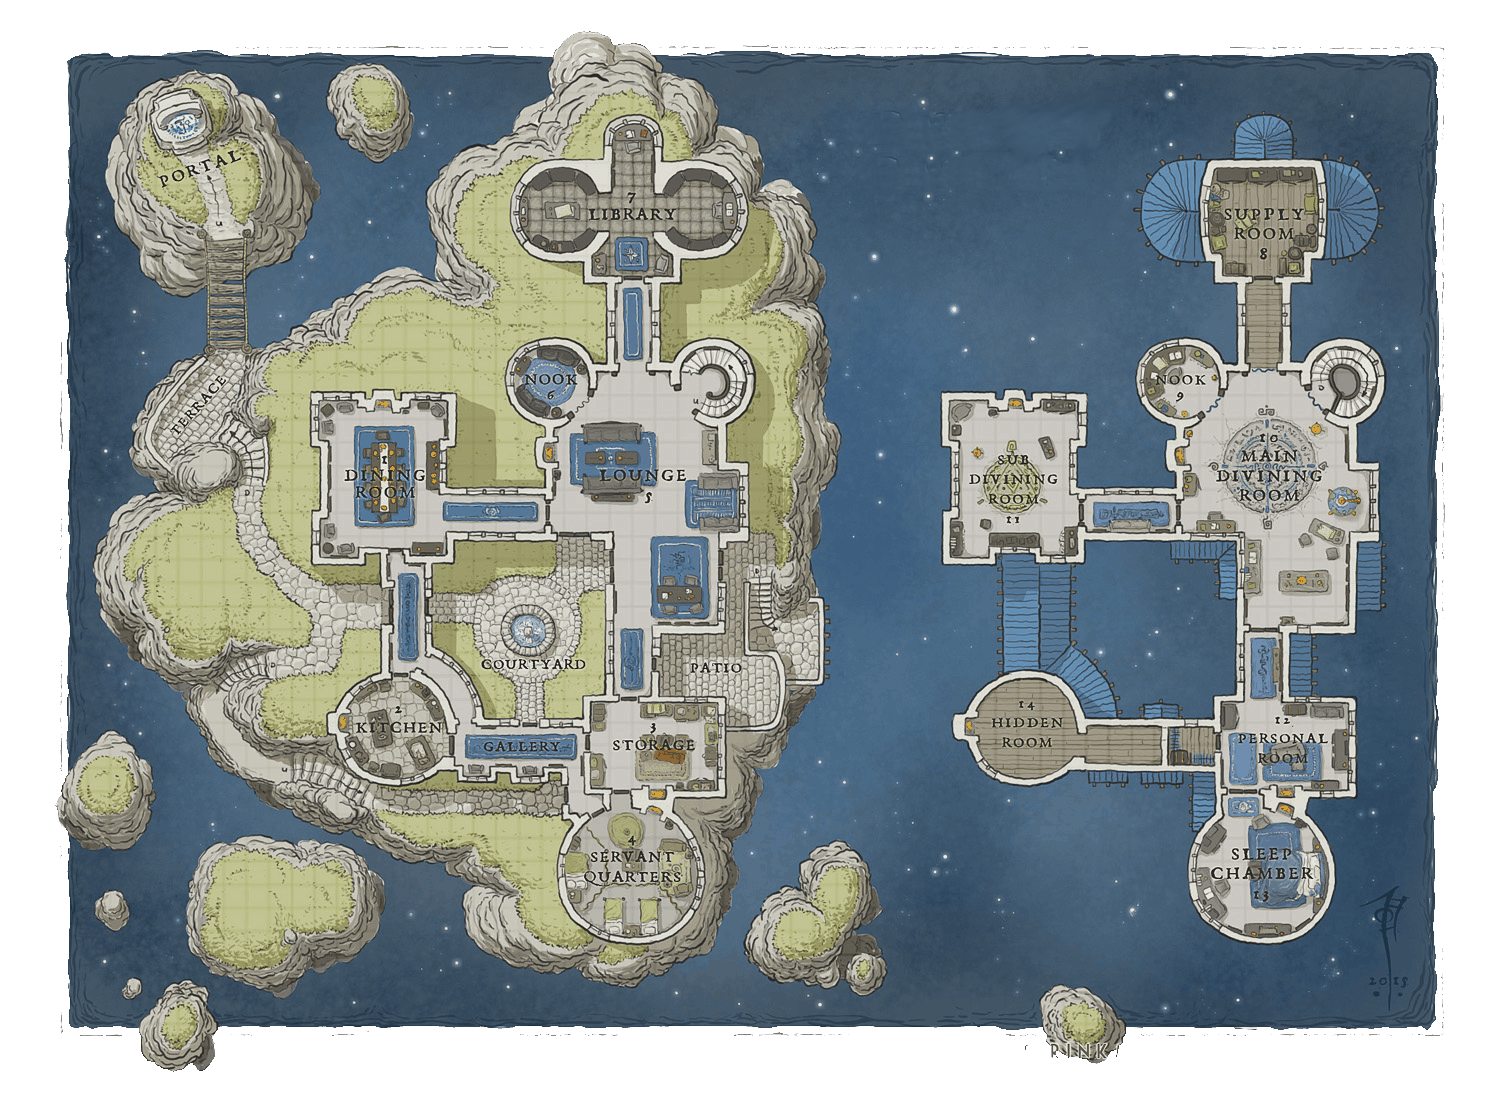
\includegraphics[width=1.05\textheight]{_img/songes-de-l-uhumele/forteresse-esseles.png}};
		\end{tikzpicture}
	\end{figure}

	\twocolumn

	\section{Bestiaire}

\subsection{Storm Trooper} \label{sec:storm-trooper}
\begin{figure}[h!]
    \centering
    
\includegraphics[height=200pt]{_img/dos-au-muur/stormtrooper.png}
\end{figure}
\paragraph{Background}
Soldats dévoué de l’empire. Certain sont des clones restant de la guerre des clones d’autres non. Ils sont entrainés au combat, équipé d’une bonne armure et armé de Fusil Blaster efficaces.

\paragraph{Traits}

\begin{itemtable}[ c c c c c ]
    \textbf{Agi} & \textbf{Int} & \textbf{\^Ame} & \textbf{For} & \textbf{Vig} \\
    d4           & d6           & d4             & d8           & d8
\end{itemtable}
\begin{itemtable}[ l X ]
    \textbf{Allure}      & 6 \\
    \textbf{Compétences} & Combat d10, Tir d10
\end{itemtable}

\paragraph{Défense}
\begin{itemtable}[ c c ]
    \textbf{Parade}     & \textbf{Résistance} \\
    7                   & 6 (+4)
\end{itemtable}

\paragraph{Attaque}
\begin{itemtable}[ X c c ]
    ~              & \textbf{Combat}   & \textbf{Dégats} \\
    Fusil Blaster  & -                 & 2d8 (3)
\end{itemtable}


\newpage


	\onecolumn
	\nocite{*}
	\printbibliography
\end{document}